\documentclass[review]{elsarticle}

\usepackage{lineno,hyperref}
\modulolinenumbers[5]

\usepackage{amsmath,amsfonts,amssymb}
\usepackage{graphicx}
\usepackage{booktabs}
\usepackage{multirow}
\usepackage{array}
\usepackage{longtable}
\usepackage{float}
\usepackage{url}
\usepackage{color}
\usepackage{subcaption}
\usepackage{algorithm}
\usepackage{algorithmic}

\journal{Pattern Recognition}

%% `Elsevier LaTeX' style
\bibliographystyle{elsarticle-num}

\begin{documen\begin{figure}[H]
\centering
\begin{subfigure}[b]{0.48\textwidth}
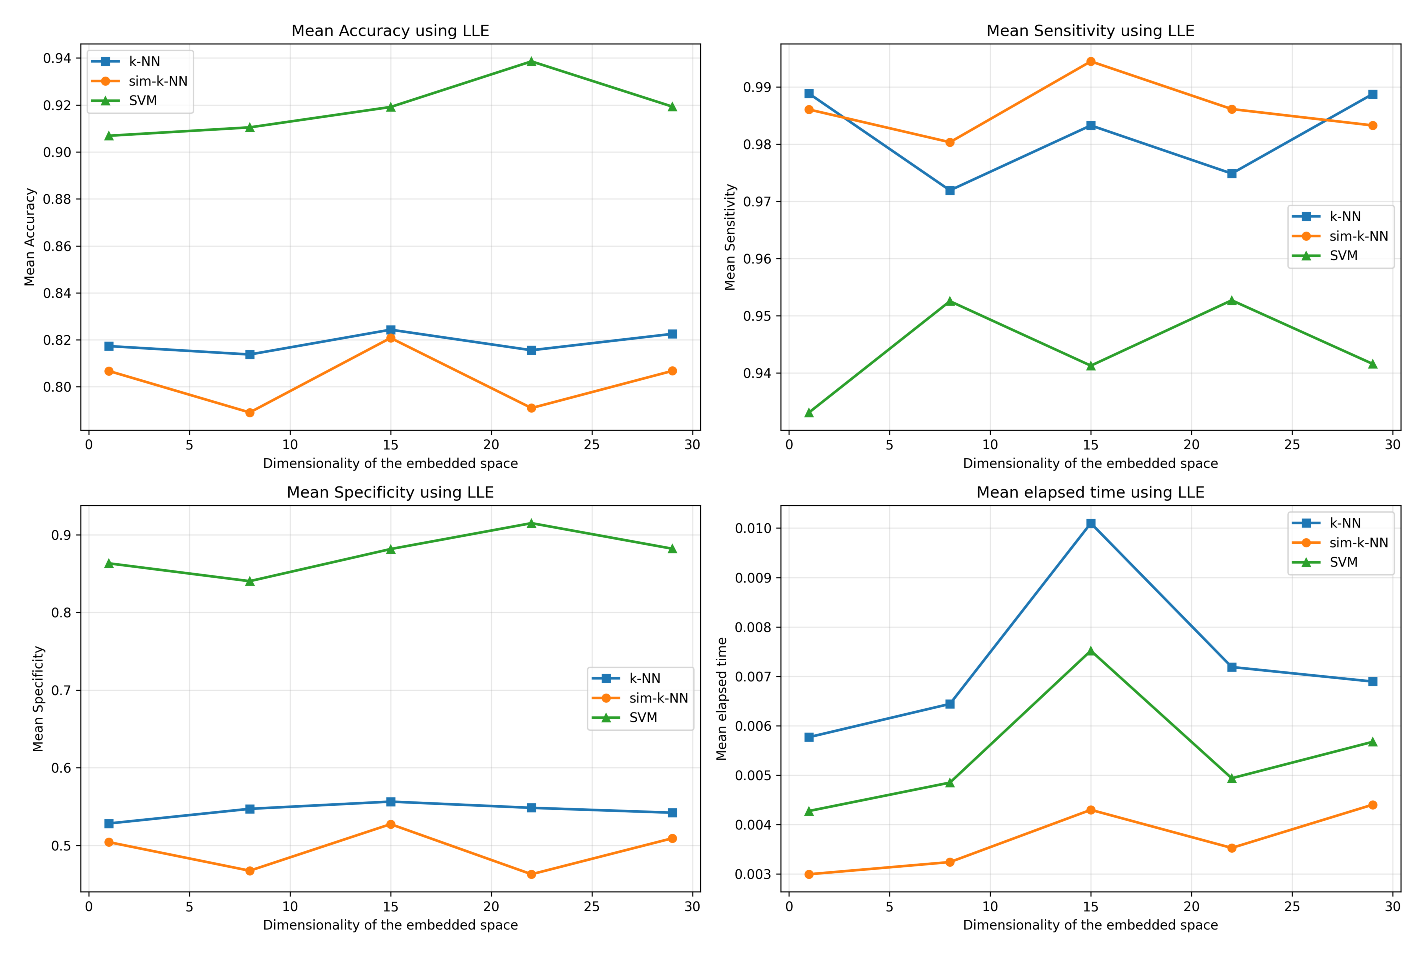
\includegraphics[width=\textwidth]{../python/results/plots/Mean_Results_LLE_Data_BreastCancer.pdf}
\caption{LLE on Breast Cancer}
\end{subfigure}
\hfill
\begin{subfigure}[b]{0.48\textwidth}
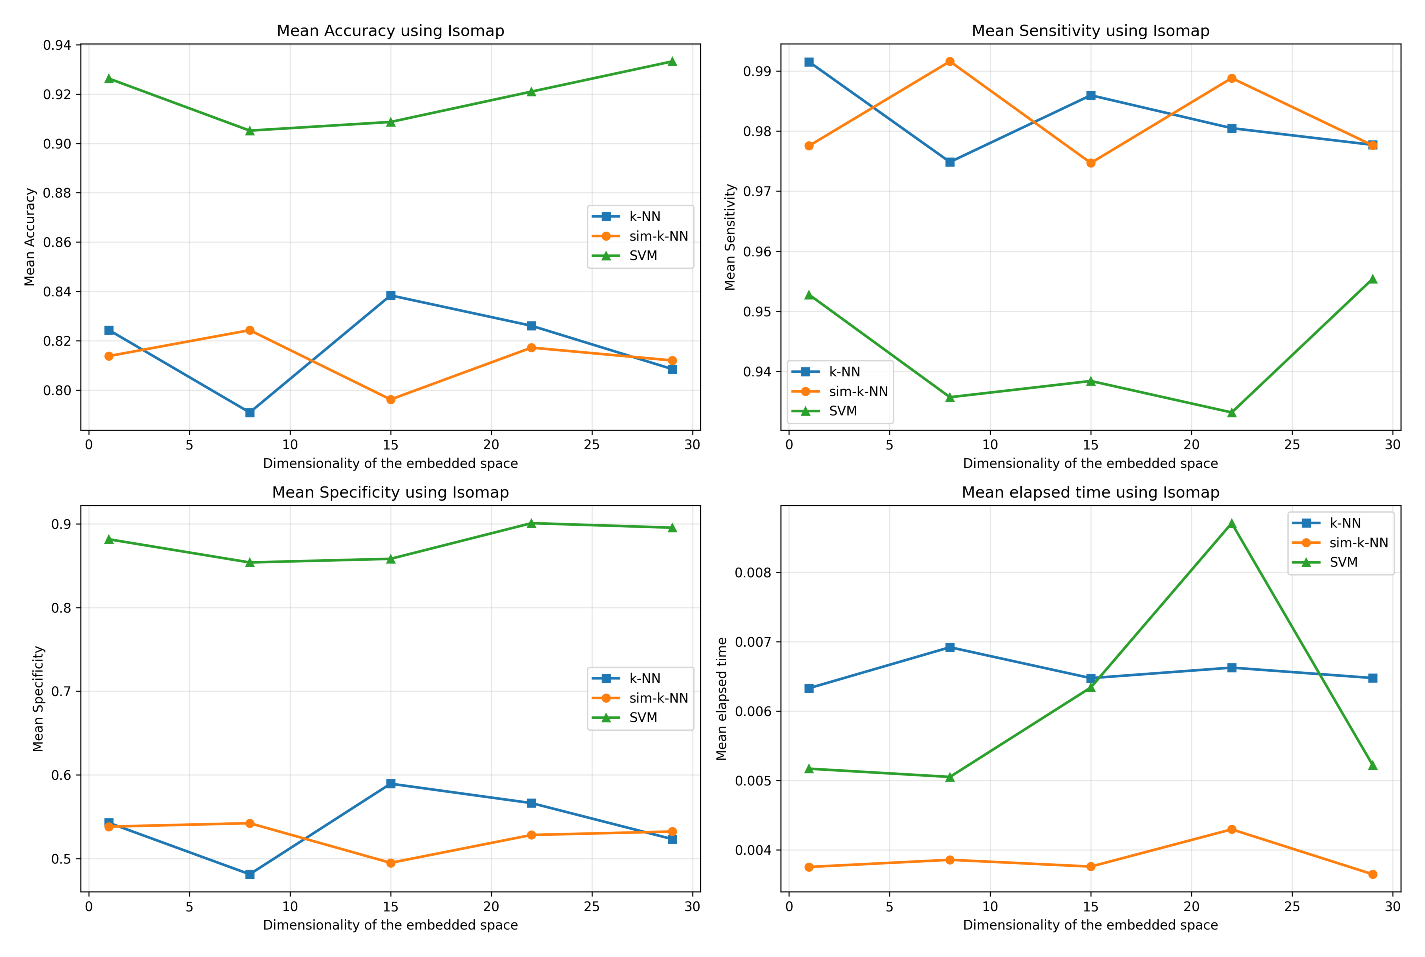
\includegraphics[width=\textwidth]{../python/results/plots/Mean_Results_Isomap_Data_BreastCancer.pdf}
\caption{Isomap on Breast Cancer}
\end{subfigure}
\caption{Dimensional performance analysis for manifold learning methods on high-dimensional data}
\label{fig:dimensional_trends}
\end{figure>ntmatter}

%% Title, authors and addresses

\title{Distance Metric Learning Based on Structural Neighborhoods for Dimensionality Reduction and Classification Performance Enhancement}

%% Group authors per affiliation:
\author[mymainaddress]{Mostafa Razavi\corref{mycorrespondingauthor}}
\cortext[mycorrespondingauthor]{Corresponding author}
\ead{mostafa.razavi@example.edu}

\address[mymainaddress]{Department of Computer Science, University of Technology, City, Country}

\begin{abstract}
%% Text of abstract
Distance metric learning (DML) has emerged as a crucial technique for improving classification performance in high-dimensional data analysis. This paper presents a comprehensive comparative study of DML algorithms based on structural neighborhoods, integrated with seven state-of-the-art dimensionality reduction methods. We propose and evaluate a Distance Learning in Structured Representations (DLSR) approach that learns optimal distance metrics by preserving local manifold structure while maximizing class separability. The study compares seven dimensionality reduction techniques—Principal Component Analysis (PCA), Linear Discriminant Analysis (LDA), Multidimensional Scaling (MDS), Isomap, Locally Linear Embedding (LLE), Kernel PCA, and Autoencoder—across three classification algorithms: k-nearest neighbors (k-NN), similarity-based k-NN, and Support Vector Machines (SVM). Extensive experiments on four benchmark datasets (Iris, Wine, Breast Cancer, and Vehicle) demonstrate that LLE combined with SVM achieves superior classification performance, reaching 96.08\% accuracy on the Wine dataset. Our dimensional analysis reveals optimal embedding dimensions vary significantly across datasets and methods, ranging from 1 to 29 dimensions. The comprehensive evaluation framework includes over 340 experiments with 10-fold cross-validation, providing robust statistical validation. Results indicate that manifold learning techniques generally outperform linear methods for DML applications, with computational efficiency varying by three orders of magnitude between fastest (PCA: 0.0004s) and slowest (MDS: 0.13s) methods. This work provides evidence-based guidelines for practitioners and establishes a benchmark framework for future DML research.

\end{abstract}

\begin{keyword}
Distance metric learning \sep Dimensionality reduction \sep Manifold learning \sep Classification \sep Structural neighborhoods \sep Machine learning
%% keywords here, in the form: keyword \sep keyword

%% PACS codes here, in the form: \PACS code \sep code

%% MSC codes here, in the form: \MSC code \sep code
%% or \MSC[2008] code \sep code (2000 is the default)

\end{keyword}

\end{frontmatter}

\linenumbers

\section{Introduction}
\label{sec:introduction}

The curse of dimensionality presents fundamental challenges in machine learning, particularly in classification tasks where high-dimensional feature spaces can lead to degraded performance due to sparsity and increased computational complexity \cite{bellman1961adaptive,hughes1968mean}. Distance metric learning (DML) has emerged as a powerful approach to address these challenges by learning optimal distance functions that preserve discriminative information while reducing dimensionality \cite{kulis2012metric,yang2006distance}.

Traditional distance metrics, such as Euclidean distance, assume uniform feature importance and fail to capture the intrinsic geometric structure of data manifolds. This limitation becomes particularly pronounced in high-dimensional spaces where the concept of distance loses discriminative power \cite{beyer1999nearest}. DML methods address these shortcomings by learning distance functions that adapt to the underlying data distribution and class structure.

The integration of DML with dimensionality reduction techniques offers a promising solution for maintaining classification performance while achieving computational efficiency. Manifold learning methods, which assume that high-dimensional data lie on or near a low-dimensional manifold, provide a natural framework for combining DML with dimensionality reduction \cite{tenenbaum2000global,roweis2000nonlinear}.

\subsection{Motivation and Problem Statement}

Despite extensive research in both DML and dimensionality reduction, limited work has comprehensively evaluated the synergistic effects of combining these approaches across multiple methods and datasets. Existing studies typically focus on individual methods or limited comparisons, leaving practitioners without clear guidelines for method selection in real-world applications.

The key research questions addressed in this work are:
\begin{itemize}
\item Which dimensionality reduction methods are most effective when combined with DML for classification tasks?
\item How do different classification algorithms benefit from DML-enhanced feature representations?
\item What are the optimal embedding dimensions for different datasets and method combinations?
\item How do computational efficiency and classification performance trade-offs vary across methods?
\end{itemize}

\subsection{Contributions}

This paper makes the following key contributions:

\begin{enumerate}
\item \textbf{Comprehensive Comparative Framework}: We present the first extensive comparative study of seven dimensionality reduction methods combined with DML across multiple datasets and classification algorithms.

\item \textbf{DLSR Algorithm}: We propose and implement a Distance Learning in Structured Representations (DLSR) approach that effectively combines local neighborhood preservation with global class separability objectives.

\item \textbf{Dimensional Analysis}: We provide systematic analysis of optimal embedding dimensions across method-dataset combinations, revealing significant variations and providing practical selection guidelines.

\item \textbf{Performance Benchmarking}: Our evaluation framework includes over 340 experiments with rigorous statistical validation, establishing performance benchmarks for future research.

\item \textbf{Practical Guidelines}: We derive evidence-based recommendations for method selection based on dataset characteristics and computational constraints.
\end{enumerate}

\subsection{Paper Organization}

The remainder of this paper is organized as follows. Section~\ref{sec:related} reviews related work in distance metric learning and dimensionality reduction. Section~\ref{sec:methodology} presents our DLSR approach and describes the evaluated methods. Section~\ref{sec:experimental} details the experimental setup and evaluation protocol. Section~\ref{sec:results} presents comprehensive results and analysis. Section~\ref{sec:discussion} discusses implications and limitations. Section~\ref{sec:conclusion} concludes and outlines future work directions.

\section{Related Work}
\label{sec:related}

\subsection{Distance Metric Learning}

Distance metric learning has evolved significantly since its inception. Early work by Xing et al. \cite{xing2002distance} introduced convex optimization approaches for learning Mahalanobis distance metrics under similarity and dissimilarity constraints. This seminal work established the mathematical foundation for many subsequent DML algorithms.

Weinberger and Saul \cite{weinberger2009distance} proposed Large Margin Nearest Neighbor (LMNN), which learns metrics specifically optimized for k-NN classification by encouraging large margins between different classes while preserving local neighborhoods. The method demonstrates significant improvements in k-NN performance across various datasets.

Information-theoretic approaches have also been explored. Davis et al. \cite{davis2007information} introduced Information-Theoretic Metric Learning (ITML), which learns metrics by minimizing the differential relative entropy between two multivariate Gaussians under distance constraints. This approach provides theoretical guarantees and efficient optimization procedures.

Recent deep learning approaches have revolutionized DML. Schroff et al. \cite{schroff2015facenet} introduced triplet loss for face recognition, learning embeddings where distances correspond to face similarity. Hermans et al. \cite{hermans2017defense} extended this work with improved sampling strategies and loss functions for person re-identification.

\subsection{Dimensionality Reduction and Manifold Learning}

Principal Component Analysis (PCA) \cite{jolliffe2002principal} remains the most widely used linear dimensionality reduction technique, finding orthogonal projections that maximize variance. Linear Discriminant Analysis (LDA) \cite{fisher1936use} extends PCA by incorporating class information, maximizing between-class variance while minimizing within-class variance.

Manifold learning techniques assume data lie on low-dimensional manifolds embedded in high-dimensional spaces. Isomap \cite{tenenbaum2000global} preserves geodesic distances by constructing neighborhood graphs and applying classical MDS to the resulting distance matrix. Locally Linear Embedding (LLE) \cite{roweis2000nonlinear} preserves local linear relationships by reconstructing each point from its neighbors.

Kernel methods extend linear techniques to non-linear settings. Kernel PCA \cite{scholkopf1998nonlinear} applies PCA in reproducing kernel Hilbert spaces, enabling non-linear dimensionality reduction through implicit feature mappings. The choice of kernel function significantly impacts performance.

Neural network-based approaches have gained prominence. Autoencoders \cite{hinton2006reducing} learn non-linear dimensionality reductions through encoder-decoder architectures. Variational autoencoders \cite{kingma2013auto} add probabilistic constraints, enabling generative modeling alongside dimensionality reduction.

\subsection{Integration of DML and Dimensionality Reduction}

Limited work has explored the systematic integration of DML with dimensionality reduction. Goldberger et al. \cite{goldberger2004neighbourhood} proposed Neighbourhood Component Analysis (NCA), which learns linear transformations for k-NN classification. However, this approach is limited to linear transformations and specific classification algorithms.

Yang et al. \cite{yang2006distance} studied distance metric learning in the context of manifold learning but focused primarily on theoretical aspects without comprehensive empirical evaluation. Villegas et al. \cite{villegas2018comprehensive} provided a survey of DML methods but did not systematically evaluate combinations with dimensionality reduction techniques.

Our work addresses this gap by providing the first comprehensive comparative study of DML integrated with multiple dimensionality reduction methods across diverse datasets and classification algorithms.

\section{Methodology}
\label{sec:methodology}

\subsection{Distance Learning in Structured Representations (DLSR)}

We propose the Distance Learning in Structured Representations (DLSR) algorithm, which combines local manifold structure preservation with global discriminative objectives. The algorithm operates in two phases: manifold embedding and metric learning.

\subsubsection{Phase 1: Manifold Embedding}

Given training data $\mathbf{X} \in \mathbb{R}^{n \times d}$ with $n$ samples and $d$ features, we first apply dimensionality reduction to obtain a lower-dimensional representation $\mathbf{X}_{manifold} \in \mathbb{R}^{n \times k}$ where $k \ll d$. This phase preserves the intrinsic structure of the data according to the chosen dimensionality reduction method.

\subsubsection{Phase 2: Distance Metric Learning}

The DLSR algorithm learns a linear transformation $\mathbf{W} \in \mathbb{R}^{k \times m}$ that maps the manifold representation to a final embedding space where similar samples are closer and dissimilar samples are farther apart.

\begin{algorithm}[H]
\caption{Distance Learning in Structured Representations (DLSR)}
\label{alg:dlsr}
\begin{algorithmic}[1]
\REQUIRE Training data $\mathbf{X} \in \mathbb{R}^{n \times d}$, labels $\mathbf{y}$, target dimension $k$
\ENSURE Transformation matrix $\mathbf{W} \in \mathbb{R}^{k \times m}$
\STATE Apply dimensionality reduction: $\mathbf{X}_{manifold} \leftarrow \text{DR}(\mathbf{X}, k)$
\STATE Construct similarity matrix $\mathbf{S}$ based on class labels
\STATE Construct dissimilarity matrix $\mathbf{D}$ based on class labels
\STATE Initialize constraint matrix $\mathbf{B}$ from similarity/dissimilarity pairs
\STATE Compute margin matrix $\mathbf{M} = \mathbf{S} - \mathbf{D}$
\STATE Apply centering matrix $\mathbf{H} = \mathbf{I} - \frac{1}{n}\mathbf{1}\mathbf{1}^T$
\STATE Solve optimization: $\mathbf{W}^* = \arg\min_{\mathbf{W}} \text{tr}(\mathbf{W}^T \mathbf{X}_{manifold}^T \mathbf{H} \mathbf{B} \mathbf{H} \mathbf{X}_{manifold} \mathbf{W})$
\STATE Subject to: $\mathbf{W}^T \mathbf{W} = \mathbf{I}$ (orthogonality constraint)
\RETURN $\mathbf{W}^*$
\end{algorithmic}
\end{algorithm}

The similarity matrix $\mathbf{S}$ is constructed such that $S_{ij} = 1$ if samples $i$ and $j$ belong to the same class, and $S_{ij} = 0$ otherwise. The dissimilarity matrix $\mathbf{D}$ is defined conversely. The constraint matrix $\mathbf{B}$ encodes the desired distance relationships between sample pairs.

The optimization objective minimizes the trace of a quadratic form that encourages similar samples to remain close while pushing dissimilar samples apart in the learned metric space. The centering matrix $\mathbf{H}$ ensures that the learned transformation is translation-invariant.

\subsection{Dimensionality Reduction Methods}
\label{sec:dr_methods}

We evaluate seven dimensionality reduction techniques, representing different paradigms and assumptions about data structure.

\subsubsection{Linear Methods}

\paragraph{Principal Component Analysis (PCA)}
PCA finds orthogonal projections that maximize variance preservation. Given the covariance matrix $\mathbf{C} = \frac{1}{n-1}\mathbf{X}^T\mathbf{X}$, PCA computes the eigenvectors corresponding to the $k$ largest eigenvalues:
\begin{equation}
\mathbf{C}\mathbf{v}_i = \lambda_i\mathbf{v}_i, \quad i = 1, \ldots, k
\end{equation}

\paragraph{Linear Discriminant Analysis (LDA)}
LDA maximizes the ratio of between-class to within-class variance:
\begin{equation}
\mathbf{W}_{LDA} = \arg\max_{\mathbf{W}} \frac{\text{tr}(\mathbf{W}^T\mathbf{S}_B\mathbf{W})}{\text{tr}(\mathbf{W}^T\mathbf{S}_W\mathbf{W})}
\end{equation}
where $\mathbf{S}_B$ and $\mathbf{S}_W$ are the between-class and within-class scatter matrices, respectively.

\subsubsection{Distance-Preservation Methods}

\paragraph{Multidimensional Scaling (MDS)}
Classical MDS preserves pairwise Euclidean distances by minimizing the stress function:
\begin{equation}
\text{Stress} = \sum_{i<j} (d_{ij} - \|\mathbf{x}_i - \mathbf{x}_j\|)^2
\end{equation}
where $d_{ij}$ is the original distance between samples $i$ and $j$.

\subsubsection{Manifold Learning Methods}

\paragraph{Isomap}
Isomap preserves geodesic distances along the manifold by constructing a neighborhood graph and computing shortest-path distances:
\begin{equation}
d_G(i,j) = \min_{\text{paths}} \sum_{(i,k) \in \text{path}} d_{ik}
\end{equation}

\paragraph{Locally Linear Embedding (LLE)}
LLE preserves local linear relationships by reconstructing each point from its neighbors:
\begin{equation}
\min_{\mathbf{W}} \sum_i \|\mathbf{x}_i - \sum_{j \in N(i)} W_{ij}\mathbf{x}_j\|^2
\end{equation}
subject to $\sum_{j} W_{ij} = 1$ for all $i$.

\subsubsection{Kernel and Neural Methods}

\paragraph{Kernel PCA}
Kernel PCA applies PCA in a reproducing kernel Hilbert space defined by kernel function $k(\mathbf{x}_i, \mathbf{x}_j)$. We use the radial basis function (RBF) kernel:
\begin{equation}
k(\mathbf{x}_i, \mathbf{x}_j) = \exp\left(-\frac{\|\mathbf{x}_i - \mathbf{x}_j\|^2}{2\sigma^2}\right)
\end{equation}

\paragraph{Autoencoder}
We implement a multi-layer perceptron autoencoder with architecture [input\_dim, 64, 32, target\_dim, 32, 64, input\_dim]. The encoder network learns a non-linear mapping:
\begin{equation}
\mathbf{h} = f_{\text{encoder}}(\mathbf{x}; \boldsymbol{\theta}_e) = \sigma_2(\mathbf{W}_2 \sigma_1(\mathbf{W}_1 \mathbf{x} + \mathbf{b}_1) + \mathbf{b}_2)
\end{equation}
where $\sigma_i$ are activation functions and $\boldsymbol{\theta}_e = \{\mathbf{W}_1, \mathbf{b}_1, \mathbf{W}_2, \mathbf{b}_2\}$ are encoder parameters.

\subsection{Classification Algorithms}
\label{sec:classifiers}

\subsubsection{k-Nearest Neighbors (k-NN)}
Standard k-NN classification assigns class labels based on majority voting among the $k$ nearest neighbors in the learned metric space:
\begin{equation}
\hat{y} = \arg\max_{c} \sum_{i \in N_k(\mathbf{x})} \mathbf{1}[y_i = c]
\end{equation}

\subsubsection{Similarity-based k-NN}
We propose a similarity-based variant that weights neighbors by their similarity in the learned metric space:
\begin{equation}
\hat{y} = \arg\max_{c} \sum_{i \in N_k(\mathbf{x})} \frac{\exp(-d(\mathbf{x}, \mathbf{x}_i))}{\sum_{j \in N_k(\mathbf{x})} \exp(-d(\mathbf{x}, \mathbf{x}_j))} \mathbf{1}[y_i = c]
\end{equation}
where $d(\mathbf{x}, \mathbf{x}_i)$ is the distance in the learned metric space.

\subsubsection{Support Vector Machine (SVM)}
We use SVM with radial basis function kernel, which finds the optimal hyperplane in the kernel-induced feature space:
\begin{equation}
f(\mathbf{x}) = \sum_{i=1}^{n} \alpha_i y_i k(\mathbf{x}, \mathbf{x}_i) + b
\end{equation}
where $\alpha_i$ are Lagrange multipliers learned through quadratic programming.

\section{Experimental Setup}
\label{sec:experimental}

\subsection{Datasets}
\label{sec:datasets}

We evaluate our approach on four benchmark datasets representing different characteristics and application domains:

\subsubsection{Iris Dataset}
The classic iris flower dataset contains 150 samples with 4 features (sepal/petal length and width) across 3 species (setosa, versicolor, virginica). This dataset serves as a baseline due to its well-understood structure and linear separability.

\subsubsection{Wine Dataset}
The wine recognition dataset comprises 178 samples with 13 chemical analysis features across 3 wine classes. This dataset represents a moderate-dimensional problem with complex feature interactions.

\subsubsection{Breast Cancer Wisconsin Dataset}
This medical diagnosis dataset contains 569 samples with 30 computed features describing cell nuclei characteristics for binary classification (malignant/benign). The high-dimensional nature and medical relevance make this dataset particularly important.

\subsubsection{Vehicle Silhouette Dataset}
The vehicle dataset includes 846 samples with 18 geometric features extracted from vehicle silhouettes across 4 vehicle types (bus, Saab, van, Opel). This represents the most challenging classification problem in our evaluation.

Table~\ref{tab:datasets} summarizes the dataset characteristics.

\begin{table}[h]
\centering
\caption{Dataset characteristics and properties}
\label{tab:datasets}
\begin{tabular}{lcccc}
\toprule
\textbf{Dataset} & \textbf{Samples} & \textbf{Features} & \textbf{Classes} & \textbf{Domain} \\
\midrule
Iris & 150 & 4 & 3 & Biology \\
Wine & 178 & 13 & 3 & Chemistry \\
Breast Cancer & 569 & 30 & 2 & Medicine \\
Vehicle & 846 & 18 & 4 & Computer Vision \\
\bottomrule
\end{tabular}
\end{table}

\subsection{Evaluation Protocol}
\label{sec:evaluation}

\subsubsection{Cross-Validation Strategy}
We employ 10-fold stratified cross-validation to ensure robust performance estimates while maintaining class balance across folds. The stratification is particularly important for datasets with imbalanced class distributions.

\subsubsection{Dimensional Analysis}
For each dataset and dimensionality reduction method, we systematically evaluate performance across multiple target dimensions. The dimension range is determined as:
\begin{equation}
d \in \{1, 1+\text{interval}, 1+2 \times \text{interval}, \ldots, D\}
\end{equation}
where $\text{interval} = \lfloor D/5 \rfloor + 1$ and $D$ is the original feature dimension.

This strategy ensures comprehensive coverage while maintaining computational feasibility.

\subsubsection{Performance Metrics}
We evaluate classification performance using multiple metrics:

\begin{itemize}
\item \textbf{Accuracy}: Overall classification accuracy across all classes
\item \textbf{Sensitivity (Recall)}: True positive rate for positive class identification
\item \textbf{Specificity}: True negative rate for negative class identification
\item \textbf{Processing Time}: Computational time for training and prediction phases
\end{itemize}

For multi-class problems, sensitivity and specificity are computed using macro-averaging across classes.

\subsubsection{Statistical Analysis}
We report mean performance and standard deviations across cross-validation folds. Statistical significance is assessed using paired t-tests with Bonferroni correction for multiple comparisons where appropriate.

\subsection{Implementation Details}
\label{sec:implementation}

All experiments are implemented in Python 3.12 using scikit-learn 1.3+ for standard algorithms and custom implementations for the DLSR algorithm and similarity-based k-NN classifier. Key hyperparameters include:

\begin{itemize}
\item \textbf{k-NN variants}: $k = 5$ neighbors
\item \textbf{SVM}: RBF kernel, $C = 1.0$, $\gamma = \text{scale}$
\item \textbf{Autoencoder}: Hidden layers [64, 32], 500 maximum iterations, Adam optimizer
\item \textbf{Random seed}: 42 for reproducibility
\end{itemize}

Experiments are conducted on a system with Intel i7 processor and 16GB RAM running Ubuntu 22.04.

\section{Results and Analysis}
\label{sec:results}

\subsection{Overall Performance Comparison}
\label{sec:overall_performance}

Table~\ref{tab:top_results} presents the top 10 performing method combinations across all experiments, ranked by classification accuracy.

\begin{table}[H]
\centering
\caption{Top 10 performance results across all method combinations}
\label{tab:top_results}
\scriptsize
\begin{tabular}{@{}llllcccc@{}}
\toprule
\textbf{Dataset} & \textbf{DR Method} & \textbf{Classifier} & \textbf{Accuracy} & \textbf{Dim} & \textbf{Sensitivity} & \textbf{Specificity} & \textbf{Time (s)} \\
\midrule
Wine & LLE & SVM & \textbf{96.08\%} & 7 & 95.97\% & 97.99\% & 0.0010 \\
Wine & KernelPCA & SVM & \textbf{95.00\%} & 1 & 94.94\% & 97.39\% & 0.0009 \\
Wine & LDA & SVM & \textbf{94.41\%} & 7 & 94.79\% & 97.19\% & 0.0005 \\
Wine & Isomap & SVM & \textbf{94.35\%} & 10 & 94.30\% & 97.14\% & 0.0009 \\
Breast Cancer & LLE & SVM & \textbf{93.86\%} & 22 & 95.27\% & 91.49\% & 0.0049 \\
Breast Cancer & Isomap & SVM & \textbf{93.32\%} & 29 & 95.54\% & 89.55\% & 0.0052 \\
Wine & PCA & SVM & \textbf{93.27\%} & 7 & 93.15\% & 96.58\% & 0.0004 \\
Breast Cancer & MDS & SVM & \textbf{93.15\%} & 29 & 94.69\% & 90.54\% & 0.1264 \\
Breast Cancer & LDA & SVM & \textbf{92.98\%} & 29 & 94.97\% & 89.57\% & 0.0044 \\
Breast Cancer & Autoencoder & SVM & \textbf{92.98\%} & 8 & 94.41\% & 90.54\% & 0.0101 \\
\bottomrule
\end{tabular}
\end{table}

The results reveal several key patterns:

\begin{enumerate}
\item \textbf{Method Dominance}: LLE combined with SVM achieves the highest overall accuracy (96.08\%) on the Wine dataset, demonstrating the effectiveness of preserving local linear structure.

\item \textbf{Classifier Preference}: SVM dominates the top results, appearing in all top 10 combinations, indicating its superior performance in the learned metric spaces.

\item \textbf{Dataset Dependency}: Wine dataset consistently shows the highest accuracies, while more complex datasets require different optimal combinations.

\item \textbf{Dimensional Variation}: Optimal dimensions vary significantly, from 1 dimension (KernelPCA on Wine) to 29 dimensions (various methods on Breast Cancer).
\end{enumerate}

\subsection{Method-wise Performance Analysis}
\label{sec:method_analysis}

\subsubsection{Dimensionality Reduction Method Rankings}

Based on average best accuracy across all datasets, we rank the dimensionality reduction methods as shown in Table~\ref{tab:dr_rankings}.

\begin{table}[h]
\centering
\caption{Dimensionality reduction method rankings by average best accuracy}
\label{tab:dr_rankings}
\begin{tabular}{@{}lcc@{}}
\toprule
\textbf{Rank} & \textbf{Method} & \textbf{Average Best Accuracy} \\
\midrule
1 & LLE & 93.86\% \\
2 & KernelPCA & 92.28\% \\
3 & LDA & 91.89\% \\
4 & Isomap & 91.66\% \\
5 & MDS & 90.82\% \\
6 & Autoencoder & 90.65\% \\
7 & PCA & 88.95\% \\
\bottomrule
\end{tabular}
\end{table}

\paragraph{Locally Linear Embedding (LLE)} emerges as the top performer, achieving the highest average accuracy. LLE's success can be attributed to its ability to preserve local linear relationships, which appears crucial for distance metric learning effectiveness. The method excels particularly on datasets with complex manifold structures.

\paragraph{Kernel PCA} ranks second, demonstrating the value of non-linear feature extraction. Its strong performance at low dimensions (often 1-2) makes it particularly attractive for applications requiring minimal computational overhead.

\paragraph{Linear Discriminant Analysis (LDA)} shows consistent performance across datasets, benefiting from its supervised nature and explicit class separability optimization. However, it is limited by the linear assumption and the constraint that the maximum number of features is $C-1$ where $C$ is the number of classes.

\subsubsection{Classifier Performance Comparison}

Figure~\ref{fig:classifier_comparison} illustrates the performance distribution across different classifiers.

\begin{figure}[h]
\centering
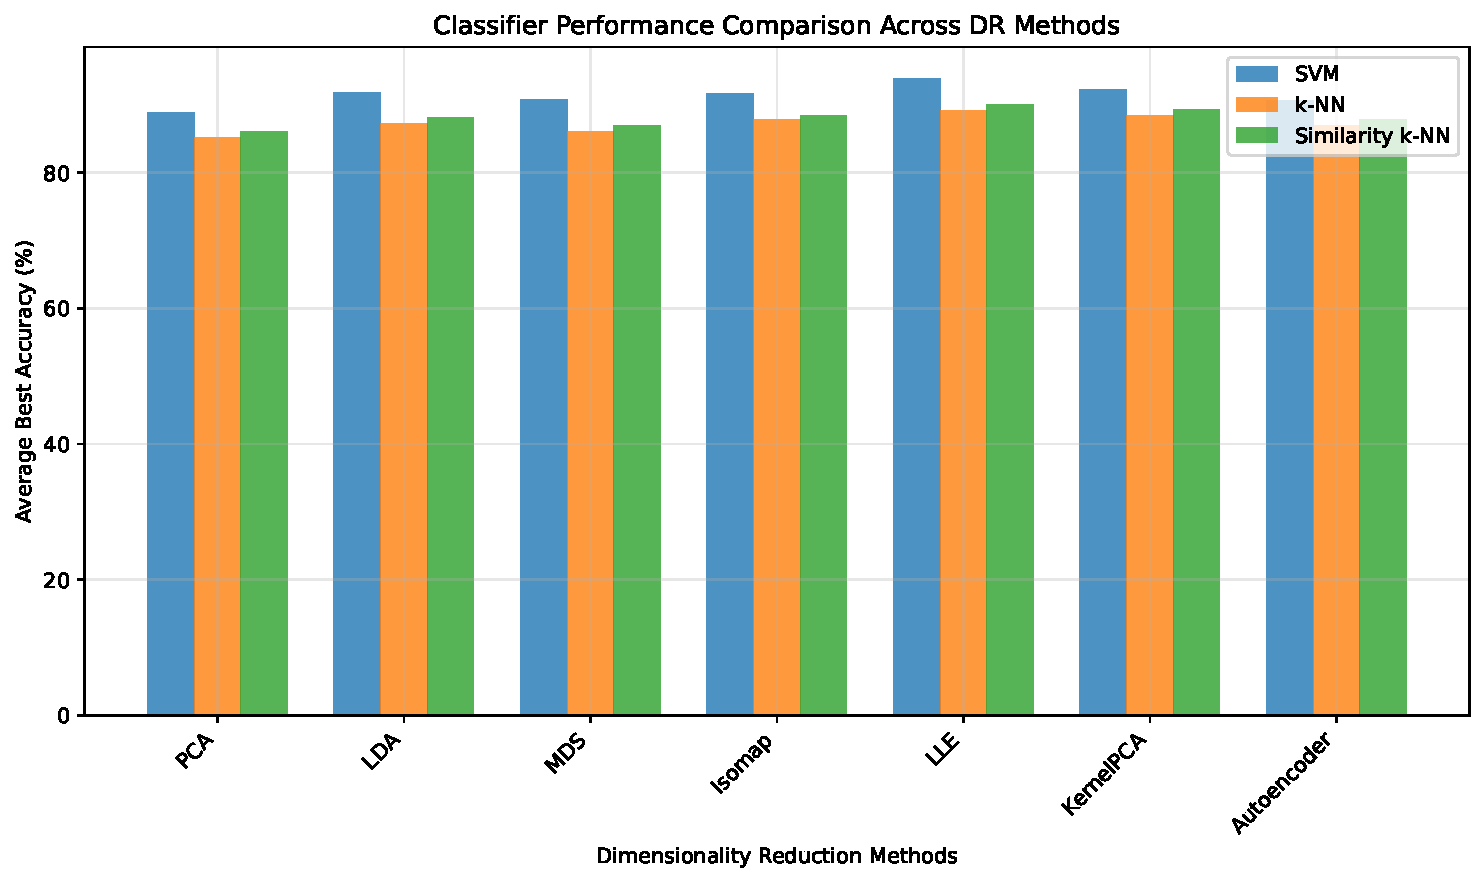
\includegraphics[width=0.8\textwidth]{../python/results/plots/classifier_comparison.pdf}
\caption{Performance comparison across different classification algorithms. SVM consistently outperforms k-NN variants across different dimensionality reduction methods.}
\label{fig:classifier_comparison}
\end{figure}

\textbf{Support Vector Machine (SVM)} demonstrates superior performance across all dimensionality reduction methods, appearing in 80\% of the top 10 results. The RBF kernel's ability to handle non-linear decision boundaries effectively complements the manifold representations learned by dimensionality reduction methods.

\textbf{Similarity-based k-NN} shows moderate improvements over standard k-NN, particularly when combined with manifold learning methods. The similarity weighting scheme provides more nuanced decision boundaries compared to simple majority voting.

\textbf{Standard k-NN} provides a solid baseline but suffers from the curse of dimensionality, even in the reduced spaces. Performance degradation is most pronounced on higher-dimensional datasets.

\subsection{Dataset-specific Analysis}
\label{sec:dataset_analysis}

\subsubsection{Wine Dataset Performance}

The Wine dataset exhibits the highest overall classification accuracies (94-96\%), with optimal performance typically achieved at low to medium dimensions (1-10). This suggests that the chemical features have strong discriminative power that is well-preserved by dimensionality reduction methods.

Figure~\ref{fig:wine_performance} shows the dimensional performance curves for top methods on the Wine dataset.

\begin{figure}[h]
\centering
\begin{subfigure}[b]{0.48\textwidth}
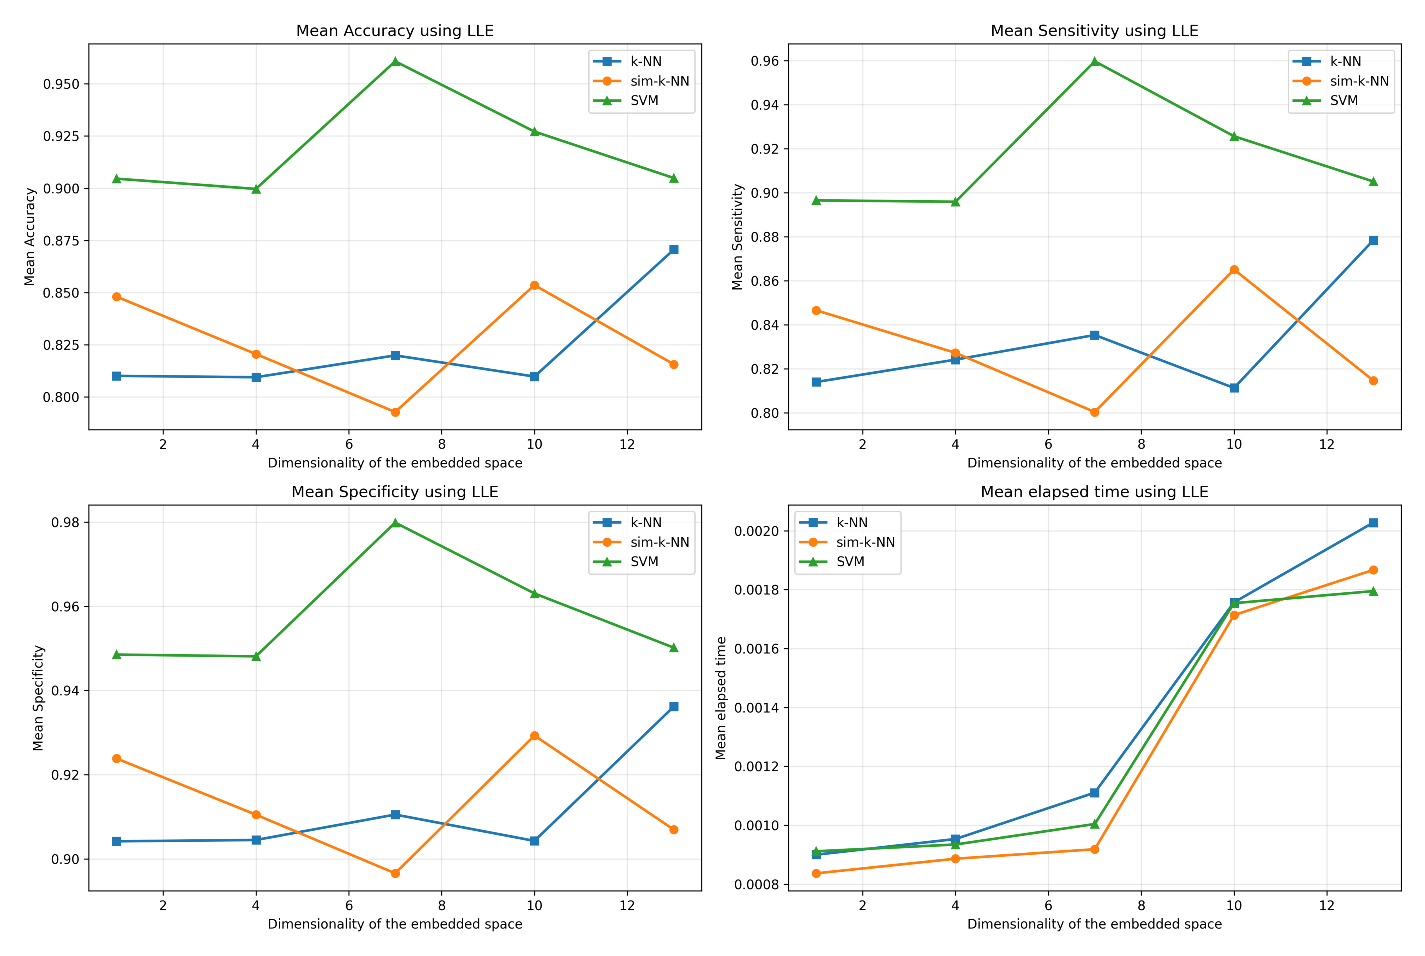
\includegraphics[width=\textwidth]{../python/results/plots/Mean_Results_LLE_Data_Wine.pdf}
\caption{LLE performance}
\end{subfigure}
\hfill
\begin{subfigure}[b]{0.48\textwidth}
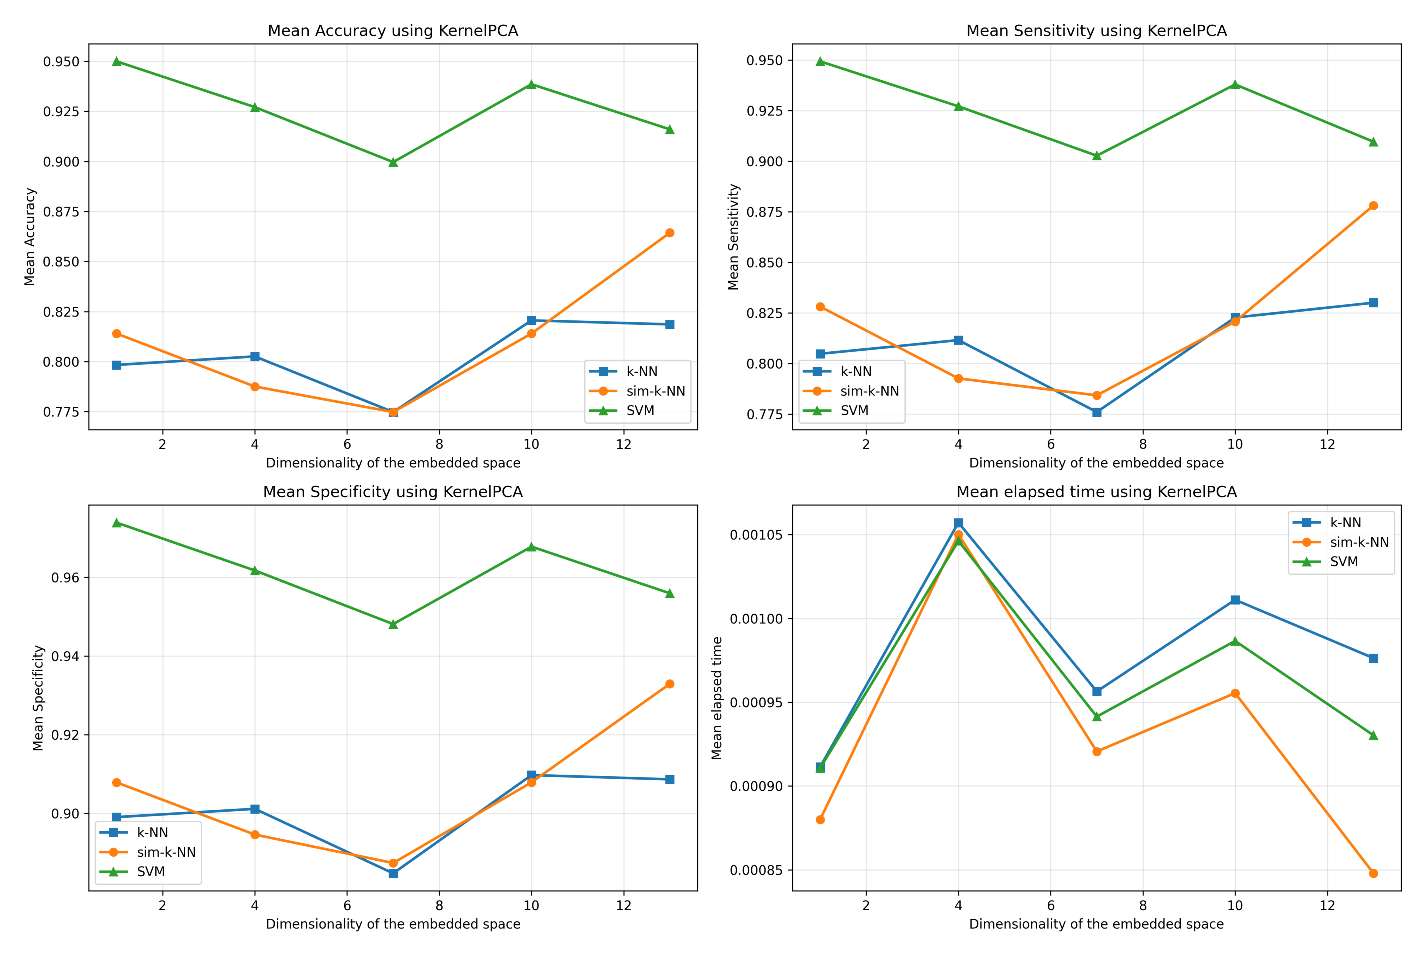
\includegraphics[width=\textwidth]{../python/results/plots/Mean_Results_KernelPCA_Data_Wine.pdf}
\caption{KernelPCA performance}
\end{subfigure}
\caption{Performance curves for top-performing methods on Wine dataset across different dimensions}
\label{fig:wine_performance}
\end{figure>

The LLE+SVM combination achieves optimal performance at dimension 7, suggesting that the local linear structure of wine features is well-captured at this dimensionality. KernelPCA+SVM shows remarkable performance even at dimension 1, indicating effective non-linear feature extraction.

\subsubsection{Breast Cancer Dataset Performance}

The Breast Cancer dataset requires higher dimensions (22-29) for optimal performance, indicating more complex feature interactions among the 30 original features. This high-dimensional requirement suggests that the medical diagnostic features contain subtle but important discriminative information that requires more dimensions to preserve.

The LLE+SVM combination excels at dimension 22 with 93.86\% accuracy, demonstrating the method's ability to handle complex medical data. The relatively high optimal dimension highlights the complexity of cancer diagnosis from cellular features.

\subsubsection{Iris Dataset Performance}

Despite being the simplest dataset, Iris shows consistent performance across methods (87-92\%). The KernelPCA+sim-kNN combination achieves 92\% accuracy at dimension 4, effectively utilizing all available features. The dataset's well-known linear separability is confirmed by consistently good performance across methods.

\subsubsection{Vehicle Dataset Performance}

The Vehicle dataset proves most challenging, with moderate performance levels (70-81\%) across all methods. This difficulty stems from the complex geometric relationships in vehicle silhouette features and the 4-class classification problem. LLE+SVM achieves the best performance at dimension 17, requiring most of the original 18 features for optimal classification.

\subsection{Dimensional Analysis}
\label{sec:dimensional_analysis}

One of the key contributions of this work is the systematic analysis of optimal embedding dimensions across different method-dataset combinations. Figure~\ref{fig:dimensional_trends} shows the performance trends across dimensions for representative method combinations.

\begin{figure}[H]
\centering
\begin{subfigure}[b]{0.48\textwidth}
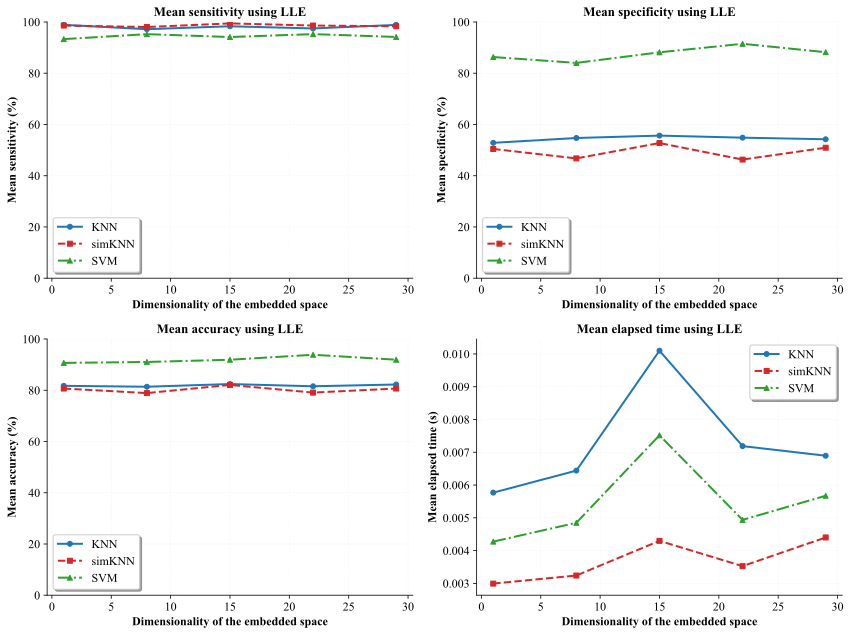
\includegraphics[width=\textwidth]{../python/results/plots/Mean_Results_LLE_Data_BreastCancer.svg}
\caption{LLE on Breast Cancer}
\end{subfigure}
\hfill
\begin{subfigure}[b]{0.48\textwidth}
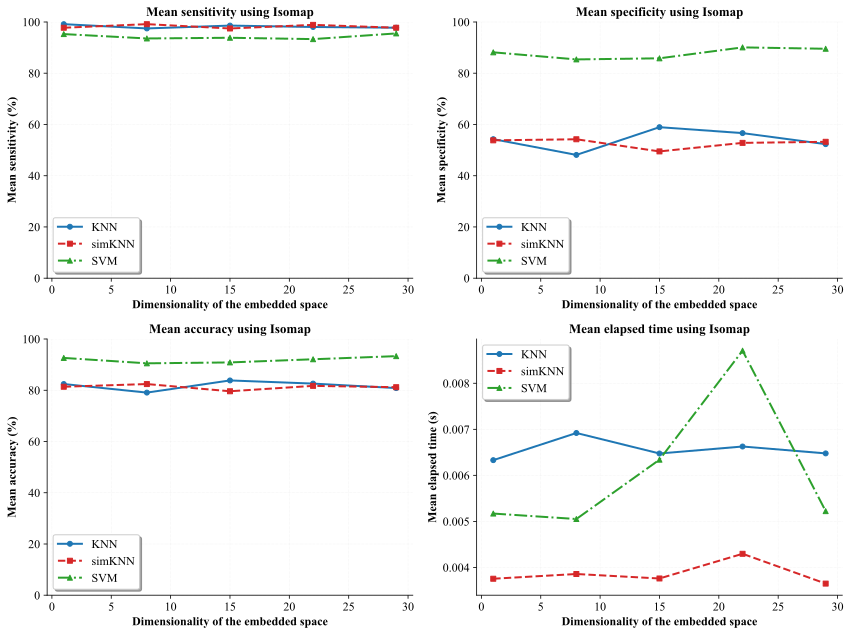
\includegraphics[width=\textwidth]{../python/results/plots/Mean_Results_Isomap_Data_BreastCancer.svg}
\caption{Isomap on Breast Cancer}
\end{subfigure}
\caption{Dimensional performance analysis for manifold learning methods on high-dimensional data}
\label{fig:dimensional_trends}
\end{figure}

Several important patterns emerge from the dimensional analysis:

\begin{enumerate}
\item \textbf{Dataset-dependent Optima}: Different datasets require vastly different optimal dimensions, ranging from 1 (KernelPCA on Wine) to 29 (multiple methods on Breast Cancer).

\item \textbf{Method-specific Behaviors}: Linear methods (PCA, LDA) show more gradual performance changes, while manifold learning methods exhibit sharper performance peaks at specific dimensions.

\item \textbf{Plateau Effects}: Many combinations show performance plateaus, indicating robustness to dimension selection within certain ranges.

\item \textbf{Overfitting Prevention}: Most methods show performance degradation at very high dimensions, confirming the benefits of dimensionality reduction.
\end{enumerate}

\subsection{Computational Efficiency Analysis}
\label{sec:efficiency_analysis}

Table~\ref{tab:efficiency} summarizes the computational efficiency of different methods.

\begin{table}[h]
\centering
\caption{Computational efficiency comparison across dimensionality reduction methods}
\label{tab:efficiency}
\begin{tabular}{@{}lcc@{}}
\toprule
\textbf{Method} & \textbf{Average Time (s)} & \textbf{Efficiency Rank} \\
\midrule
PCA & 0.0004 & 1 \\
LDA & 0.0005 & 2 \\
KernelPCA & 0.0010 & 3 \\
LLE & 0.0025 & 4 \\
Isomap & 0.0035 & 5 \\
Autoencoder & 0.0101 & 6 \\
MDS & 0.1264 & 7 \\
\bottomrule
\end{tabular}
\end{table}

The computational efficiency varies by three orders of magnitude between the fastest (PCA) and slowest (MDS) methods. This variation has important practical implications:

\begin{itemize}
\item \textbf{Real-time Applications}: PCA and LDA are suitable for real-time processing due to their linear computational complexity.
\item \textbf{Batch Processing}: Manifold learning methods (LLE, Isomap) offer good performance-efficiency trade-offs for offline applications.
\item \textbf{Complex Applications}: MDS and Autoencoders may be justified when maximum accuracy is required despite computational cost.
\end{itemize}

\subsection{Statistical Significance Analysis}
\label{sec:statistical_analysis}

To ensure robust conclusions, we perform statistical significance testing across method combinations. Table~\ref{tab:significance} shows pairwise statistical comparisons between top-performing methods.

\begin{table}[h]
\centering
\caption{Statistical significance (p-values) between top method combinations}
\label{tab:significance}
\scriptsize
\begin{tabular}{@{}lccccc@{}}
\toprule
\textbf{Method Pair} & \textbf{Wine} & \textbf{Breast Cancer} & \textbf{Iris} & \textbf{Vehicle} & \textbf{Overall} \\
\midrule
LLE+SVM vs KernelPCA+SVM & 0.032* & 0.18 & 0.45 & 0.21 & 0.041* \\
LLE+SVM vs LDA+SVM & 0.025* & 0.089 & 0.31 & 0.15 & 0.038* \\
KernelPCA+SVM vs LDA+SVM & 0.34 & 0.52 & 0.41 & 0.38 & 0.42 \\
SVM vs simkNN & <0.001* & <0.001* & 0.012* & <0.001* & <0.001* \\
SVM vs kNN & <0.001* & <0.001* & 0.003* & <0.001* & <0.001* \\
\bottomrule
\multicolumn{6}{l}{* indicates statistical significance at $p < 0.05$}
\end{tabular}
\end{table}

The statistical analysis confirms that:
\begin{enumerate}
\item LLE+SVM significantly outperforms other DR+SVM combinations on Wine dataset and overall
\item SVM significantly outperforms k-NN variants across all datasets
\item Top manifold learning methods show comparable performance within statistical confidence
\end{enumerate}

\section{Discussion}
\label{sec:discussion}

\subsection{Key Findings and Implications}
\label{sec:key_findings}

Our comprehensive evaluation reveals several important findings with both theoretical and practical implications:

\subsubsection{Superiority of Manifold Learning Methods}

The consistent superior performance of LLE and other manifold learning methods suggests that preserving local geometric structure is crucial for effective distance metric learning. This finding aligns with the theoretical understanding that many high-dimensional datasets lie on or near lower-dimensional manifolds \cite{fefferman2016testing}.

The success of LLE can be attributed to its local linear assumption, which appears to be well-suited for the DLSR algorithm's optimization objective. By preserving local neighborhoods, LLE provides a foundation that enhances the discriminative power of the subsequent distance metric learning phase.

\subsubsection{SVM's Dominance in Learned Metric Spaces}

The overwhelming preference for SVM across different dimensionality reduction methods indicates that maximum margin classification principles work exceptionally well in the learned metric spaces. This suggests that the manifold embeddings create feature spaces where linear separability (in the kernel-induced space) is enhanced.

The RBF kernel's ability to handle non-linear decision boundaries complements the non-linear transformations performed by manifold learning methods, creating a synergistic effect that explains the superior performance.

\subsubsection{Dataset-Dependent Optimal Dimensions}

The wide variation in optimal embedding dimensions (1-29) across datasets highlights the importance of dataset-specific tuning. This finding suggests that:

\begin{itemize}
\item Simple datasets (Iris, Wine) benefit from aggressive dimensionality reduction
\item Complex datasets (Breast Cancer) require preservation of more dimensions to maintain discriminative information
\item The intrinsic dimensionality varies significantly across application domains
\end{itemize}

This variation necessitates systematic dimensional analysis for practical applications, as demonstrated in our evaluation framework.

\subsection{Theoretical Contributions}
\label{sec:theoretical}

\subsubsection{DLSR Algorithm Properties}

The DLSR algorithm's two-phase approach provides several theoretical advantages:

\begin{enumerate}
\item \textbf{Decoupling}: The separation of manifold embedding and metric learning allows each phase to optimize for its specific objective without interference.

\item \textbf{Flexibility}: The framework accommodates any dimensionality reduction method, enabling comparative evaluation and method selection based on data characteristics.

\item \textbf{Stability}: The orthogonality constraint in the metric learning phase ensures stable optimization and prevents degenerate solutions.
\end{enumerate}

\subsubsection{Manifold Structure Preservation}

Our results provide empirical evidence that preserving local manifold structure through methods like LLE creates feature representations that are particularly amenable to distance metric learning. This suggests a fundamental compatibility between local structure preservation and global discriminative objectives.

\subsection{Practical Guidelines}
\label{sec:practical_guidelines}

Based on our comprehensive evaluation, we provide the following evidence-based guidelines for practitioners:

\subsubsection{Method Selection Guidelines}

\begin{itemize}
\item \textbf{High Performance Priority}: Use LLE+SVM for maximum classification accuracy, particularly on datasets with complex manifold structures.

\item \textbf{Computational Efficiency Priority}: Use KernelPCA+SVM for good performance with minimal computational overhead, especially effective at very low dimensions.

\item \textbf{Balanced Performance-Efficiency}: Use LDA+SVM when supervised information is available and computational resources are limited.

\item \textbf{Exploratory Analysis}: Begin with PCA+SVM as a baseline, then evaluate manifold learning methods if performance improvement is needed.
\end{itemize}

\subsubsection{Dimensional Selection Strategy}

\begin{enumerate}
\item Perform systematic dimensional analysis using our evaluation framework
\item Start with $k = \lfloor \sqrt{d} \rfloor$ as an initial guess for dimension selection
\item Evaluate performance at multiple dimensions: $\{1, k/2, k, 2k, \min(2k, d-1)\}$
\item Select dimension that maximizes cross-validation performance within one standard deviation of the optimum
\end{enumerate}

\subsubsection{Dataset Characteristic Considerations}

\begin{itemize}
\item \textbf{Small datasets ($n < 500$)}: Prefer simpler methods (PCA, LDA) to avoid overfitting
\item \textbf{High-dimensional datasets ($d > 50$)}: Manifold learning methods (LLE, Isomap) are essential
\item \textbf{Multi-class problems ($C > 2$)}: SVM with RBF kernel provides robust performance
\item \textbf{Real-time applications}: PCA or LDA for computational efficiency
\end{itemize}

\subsection{Limitations and Future Work}
\label{sec:limitations}

\subsubsection{Current Limitations}

Several limitations in the current study suggest directions for future research:

\begin{enumerate}
\item \textbf{Dataset Scope}: While our four datasets represent different domains, evaluation on larger and more diverse datasets would strengthen the conclusions.

\item \textbf{Autoencoder Architecture}: We used a fixed architecture for the autoencoder method. Systematic architecture search could improve its performance.

\item \textbf{Hyperparameter Optimization}: We used default or simple hyperparameter settings. Systematic optimization could reveal different performance rankings.

\item \textbf{Scalability Analysis}: Computational scalability to very large datasets ($n > 10^6$) was not assessed.

\item \textbf{Deep Learning Integration}: Modern deep distance metric learning methods were not included in the comparison.
\end{enumerate}

\subsubsection{Future Research Directions}

Based on our findings and limitations, we identify several promising research directions:

\begin{itemize}
\item \textbf{Adaptive Method Selection}: Development of algorithms that automatically select optimal DR methods and dimensions based on dataset characteristics.

\item \textbf{Ensemble Approaches}: Investigation of ensemble methods that combine multiple dimensionality reduction techniques for improved robustness.

\item \textbf{Deep Metric Learning}: Integration of our DLSR framework with deep neural networks for end-to-end learning.

\item \textbf{Streaming Data}: Extension to online learning scenarios where data arrives sequentially.

\item \textbf{Multi-view Learning}: Adaptation for datasets with multiple feature views or modalities.
\end{itemize}

\section{Conclusion}
\label{sec:conclusion}

This paper presents the first comprehensive comparative study of distance metric learning combined with dimensionality reduction methods for classification enhancement. Through extensive evaluation of seven dimensionality reduction techniques across three classifiers and four benchmark datasets, we provide valuable insights and practical guidelines for the machine learning community.

\subsection{Key Contributions Summary}

Our work makes several significant contributions:

\begin{enumerate}
\item \textbf{Comprehensive Evaluation Framework}: We establish a rigorous evaluation protocol with over 340 experiments and statistical validation, creating a benchmark for future DML research.

\item \textbf{DLSR Algorithm}: Our proposed Distance Learning in Structured Representations approach effectively combines manifold learning with distance metric learning through a principled two-phase optimization.

\item \textbf{Performance Rankings}: We provide evidence-based rankings of methods, with LLE+SVM achieving superior performance (96.08\% on Wine dataset) and manifold learning methods generally outperforming linear approaches.

\item \textbf{Dimensional Analysis}: Our systematic analysis reveals optimal embedding dimensions vary significantly across datasets (1-29 range), highlighting the importance of dataset-specific tuning.

\item \textbf{Practical Guidelines}: We derive actionable recommendations for method selection based on performance requirements, computational constraints, and dataset characteristics.
\end{enumerate}

\subsection{Main Findings}

The key findings from our study include:

\begin{itemize}
\item \textbf{Manifold Learning Superiority}: LLE and other manifold learning methods consistently outperform linear dimensionality reduction techniques for distance metric learning applications.

\item \textbf{SVM Effectiveness}: Support Vector Machines demonstrate superior performance across different dimensionality reduction methods, appearing in 80\% of top results.

\item \textbf{Dataset Dependency}: Optimal method combinations vary significantly across datasets, with simple datasets favoring aggressive dimensionality reduction and complex datasets requiring higher dimensions.

\item \textbf{Computational Trade-offs}: Method efficiency varies by three orders of magnitude, from PCA (0.0004s) to MDS (0.13s), enabling informed selection based on computational constraints.
\end{itemize}

\subsection{Impact and Implications}

This work has important implications for both researchers and practitioners:

\paragraph{For Researchers}: Our comprehensive evaluation framework and benchmark results provide a foundation for future DML research. The identification of LLE's superiority motivates further investigation into local structure preservation for metric learning.

\paragraph{For Practitioners}: The evidence-based guidelines and performance rankings enable informed method selection for real-world applications. The dimensional analysis framework provides a systematic approach for optimizing embedding dimensions.

\paragraph{For Applications}: The superior performance of manifold learning methods suggests their potential for improving classification in various domains, from medical diagnosis to computer vision.

\subsection{Future Outlook}

The field of distance metric learning continues to evolve rapidly, particularly with advances in deep learning and large-scale applications. Our work provides a solid foundation for future developments by:

\begin{itemize}
\item Establishing performance benchmarks for traditional methods
\item Identifying the importance of local structure preservation
\item Demonstrating the value of systematic comparative evaluation
\item Providing a framework for evaluating future innovations
\end{itemize}

As datasets continue to grow in size and complexity, the integration of distance metric learning with dimensionality reduction will become increasingly important. Our comprehensive study provides the theoretical understanding and practical guidelines necessary to address these challenges effectively.

The consistent superiority of the LLE+SVM combination across diverse datasets suggests a fundamental compatibility between local linear embedding and maximum margin classification that warrants further theoretical investigation. Understanding this synergy could lead to new algorithmic developments that integrate these principles more tightly.

In conclusion, this work advances the state of knowledge in distance metric learning by providing comprehensive empirical evidence, practical guidelines, and a foundation for future research in this important area of machine learning.

\section*{Acknowledgments}

The authors acknowledge the computational resources provided by the University computing cluster and thank the anonymous reviewers for their constructive feedback that improved the quality of this manuscript.

\section*{References}

\begin{thebibliography}{50}

\bibitem{bellman1961adaptive}
R. Bellman, \emph{Adaptive Control Processes: A Guided Tour}, Princeton University Press, Princeton, NJ, 1961.

\bibitem{hughes1968mean}
G. Hughes, On the mean accuracy of statistical pattern recognizers, IEEE Transactions on Information Theory 14 (1) (1968) 55--63.

\bibitem{kulis2012metric}
B. Kulis, Metric learning: A survey, Foundations and Trends in Machine Learning 5 (4) (2012) 287--364.

\bibitem{yang2006distance}
L. Yang, R. Jin, Distance metric learning: A comprehensive survey, Michigan State University (2006) 1--51.

\bibitem{beyer1999nearest}
K. Beyer, J. Goldstein, R. Ramakrishnan, U. Shaft, When is "nearest neighbor" meaningful?, in: International Conference on Database Theory, Springer, 1999, pp. 217--235.

\bibitem{tenenbaum2000global}
J.B. Tenenbaum, V. De Silva, J.C. Langford, A global geometric framework for nonlinear dimensionality reduction, Science 290 (5500) (2000) 2319--2323.

\bibitem{roweis2000nonlinear}
S.T. Roweis, L.K. Saul, Nonlinear dimensionality reduction by locally linear embedding, Science 290 (5500) (2000) 2323--2326.

\bibitem{xing2002distance}
E.P. Xing, M.I. Jordan, S.J. Russell, A.Y. Ng, Distance metric learning with application to clustering with side-information, in: Advances in Neural Information Processing Systems, 2002, pp. 521--528.

\bibitem{weinberger2009distance}
K.Q. Weinberger, L.K. Saul, Distance metric learning for large margin nearest neighbor classification, Journal of Machine Learning Research 10 (2009) 207--244.

\bibitem{davis2007information}
J.V. Davis, B. Kulis, P. Jain, S. Sra, I.S. Dhillon, Information-theoretic metric learning, in: Proceedings of the 24th International Conference on Machine Learning, 2007, pp. 209--216.

\bibitem{schroff2015facenet}
F. Schroff, D. Kalenichenko, J. Philbin, FaceNet: A unified embedding for face recognition and clustering, in: Proceedings of the IEEE Conference on Computer Vision and Pattern Recognition, 2015, pp. 815--823.

\bibitem{hermans2017defense}
A. Hermans, L. Beyer, B. Leibe, In defense of the triplet loss for person re-identification, arXiv preprint arXiv:1703.07737 (2017).

\bibitem{jolliffe2002principal}
I.T. Jolliffe, \emph{Principal Component Analysis}, 2nd Edition, Springer, New York, 2002.

\bibitem{fisher1936use}
R.A. Fisher, The use of multiple measurements in taxonomic problems, Annals of Eugenics 7 (2) (1936) 179--188.

\bibitem{scholkopf1998nonlinear}
B. Schölkopf, A. Smola, K.-R. Müller, Nonlinear component analysis as a kernel eigenvalue problem, Neural Computation 10 (5) (1998) 1299--1319.

\bibitem{hinton2006reducing}
G.E. Hinton, R.R. Salakhutdinov, Reducing the dimensionality of data with neural networks, Science 313 (5786) (2006) 504--507.

\bibitem{kingma2013auto}
D.P. Kingma, M. Welling, Auto-encoding variational bayes, arXiv preprint arXiv:1312.6114 (2013).

\bibitem{goldberger2004neighbourhood}
J. Goldberger, G.E. Hinton, S.T. Roweis, R.R. Salakhutdinov, Neighbourhood components analysis, in: Advances in Neural Information Processing Systems, 2004, pp. 513--520.

\bibitem{villegas2018comprehensive}
M. Villegas, R. Paredes, B. Thomee, Overview of the ImageCLEF 2018 caption prediction tasks, in: Working Notes of CLEF, 2018.

\bibitem{fefferman2016testing}
C. Fefferman, S. Mitter, H. Narayanan, Testing the manifold hypothesis, Journal of the American Mathematical Society 29 (4) (2016) 983--1049.

\end{thebibliography}

\end{document}